\documentclass[1p]{elsarticle_modified}
%\bibliographystyle{elsarticle-num}

%\usepackage[colorlinks]{hyperref}
%\usepackage{abbrmath_seonhwa} %\Abb, \Ascr, \Acal ,\Abf, \Afrak
\usepackage{amsfonts}
\usepackage{amssymb}
\usepackage{amsmath}
\usepackage{amsthm}
\usepackage{scalefnt}
\usepackage{amsbsy}
\usepackage{kotex}
\usepackage{caption}
\usepackage{subfig}
\usepackage{color}
\usepackage{graphicx}
\usepackage{xcolor} %% white, black, red, green, blue, cyan, magenta, yellow
\usepackage{float}
\usepackage{setspace}
\usepackage{hyperref}

\usepackage{tikz}
\usetikzlibrary{arrows}

\usepackage{multirow}
\usepackage{array} % fixed length table
\usepackage{hhline}

%%%%%%%%%%%%%%%%%%%%%
\makeatletter
\renewcommand*\env@matrix[1][\arraystretch]{%
	\edef\arraystretch{#1}%
	\hskip -\arraycolsep
	\let\@ifnextchar\new@ifnextchar
	\array{*\c@MaxMatrixCols c}}
\makeatother %https://tex.stackexchange.com/questions/14071/how-can-i-increase-the-line-spacing-in-a-matrix
%%%%%%%%%%%%%%%

\usepackage[normalem]{ulem}

\newcommand{\msout}[1]{\ifmmode\text{\sout{\ensuremath{#1}}}\else\sout{#1}\fi}
%SOURCE: \msout is \stkout macro in https://tex.stackexchange.com/questions/20609/strikeout-in-math-mode

\newcommand{\cancel}[1]{
	\ifmmode
	{\color{red}\msout{#1}}
	\else
	{\color{red}\sout{#1}}
	\fi
}

\newcommand{\add}[1]{
	{\color{blue}\uwave{#1}}
}

\newcommand{\replace}[2]{
	\ifmmode
	{\color{red}\msout{#1}}{\color{blue}\uwave{#2}}
	\else
	{\color{red}\sout{#1}}{\color{blue}\uwave{#2}}
	\fi
}

\newcommand{\Sol}{\mathcal{S}} %segment
\newcommand{\D}{D} %diagram
\newcommand{\A}{\mathcal{A}} %arc


%%%%%%%%%%%%%%%%%%%%%%%%%%%%%5 test

\def\sl{\operatorname{\textup{SL}}(2,\Cbb)}
\def\psl{\operatorname{\textup{PSL}}(2,\Cbb)}
\def\quan{\mkern 1mu \triangleright \mkern 1mu}

\theoremstyle{definition}
\newtheorem{thm}{Theorem}[section]
\newtheorem{prop}[thm]{Proposition}
\newtheorem{lem}[thm]{Lemma}
\newtheorem{ques}[thm]{Question}
\newtheorem{cor}[thm]{Corollary}
\newtheorem{defn}[thm]{Definition}
\newtheorem{exam}[thm]{Example}
\newtheorem{rmk}[thm]{Remark}
\newtheorem{alg}[thm]{Algorithm}

\newcommand{\I}{\sqrt{-1}}
\begin{document}

%\begin{frontmatter}
%
%\title{Boundary parabolic representations of knots up to 8 crossings}
%
%%% Group authors per affiliation:
%\author{Yunhi Cho} 
%\address{Department of Mathematics, University of Seoul, Seoul, Korea}
%\ead{yhcho@uos.ac.kr}
%
%
%\author{Seonhwa Kim} %\fnref{s_kim}}
%\address{Center for Geometry and Physics, Institute for Basic Science, Pohang, 37673, Korea}
%\ead{ryeona17@ibs.re.kr}
%
%\author{Hyuk Kim}
%\address{Department of Mathematical Sciences, Seoul National University, Seoul 08826, Korea}
%\ead{hyukkim@snu.ac.kr}
%
%\author{Seokbeom Yoon}
%\address{Department of Mathematical Sciences, Seoul National University, Seoul, 08826,  Korea}
%\ead{sbyoon15@snu.ac.kr}
%
%\begin{abstract}
%We find all boundary parabolic representation of knots up to 8 crossings.
%
%\end{abstract}
%\begin{keyword}
%    \MSC[2010] 57M25 
%\end{keyword}
%
%\end{frontmatter}

%\linenumbers
%\tableofcontents
%
\newcommand\colored[1]{\textcolor{white}{\rule[-0.35ex]{0.8em}{1.4ex}}\kern-0.8em\color{red} #1}%
%\newcommand\colored[1]{\textcolor{white}{ #1}\kern-2.17ex	\textcolor{white}{ #1}\kern-1.81ex	\textcolor{white}{ #1}\kern-2.15ex\color{red}#1	}

{\Large $\underline{12n_{0652}~(K12n_{0652})}$}

\setlength{\tabcolsep}{10pt}
\renewcommand{\arraystretch}{1.6}
\vspace{1cm}\begin{tabular}{m{100pt}>{\centering\arraybackslash}m{274pt}}
\multirow{5}{120pt}{
	\centering
	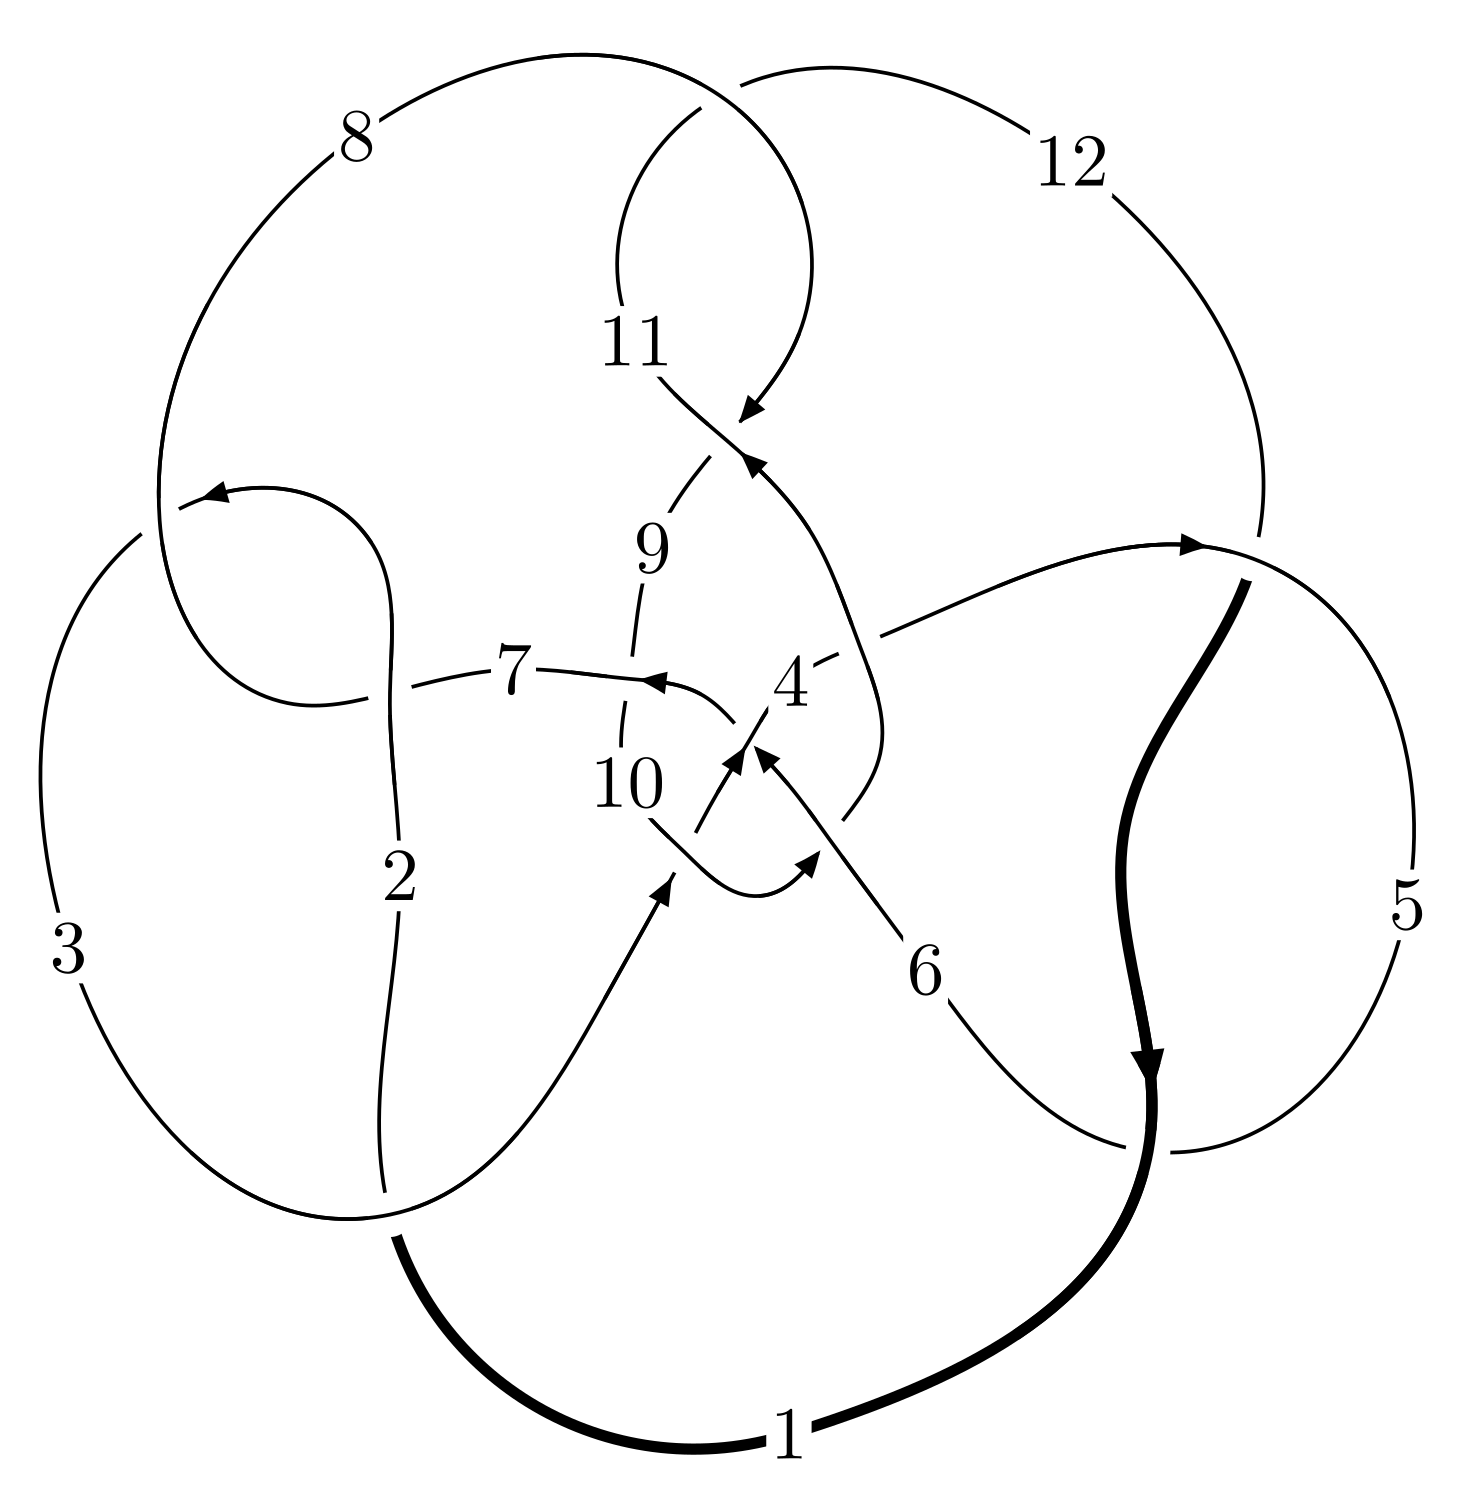
\includegraphics[width=112pt]{../../../GIT/diagram.site/Diagrams/png/2741_12n_0652.png}\\
\ \ \ A knot diagram\footnotemark}&
\allowdisplaybreaks
\textbf{Linearized knot diagam} \\
\cline{2-2}
 &
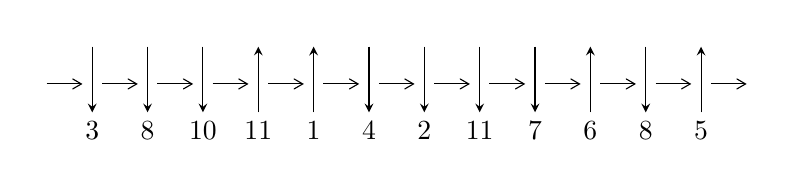
\begin{tikzpicture}[x=20pt, y=17pt]
	% nodes
	\node (C0) at (0, 0) {};
	\node (C1) at (1, 0) {};
	\node (C1U) at (1, +1) {};
	\node (C1D) at (1, -1) {3};

	\node (C2) at (2, 0) {};
	\node (C2U) at (2, +1) {};
	\node (C2D) at (2, -1) {8};

	\node (C3) at (3, 0) {};
	\node (C3U) at (3, +1) {};
	\node (C3D) at (3, -1) {10};

	\node (C4) at (4, 0) {};
	\node (C4U) at (4, +1) {};
	\node (C4D) at (4, -1) {11};

	\node (C5) at (5, 0) {};
	\node (C5U) at (5, +1) {};
	\node (C5D) at (5, -1) {1};

	\node (C6) at (6, 0) {};
	\node (C6U) at (6, +1) {};
	\node (C6D) at (6, -1) {4};

	\node (C7) at (7, 0) {};
	\node (C7U) at (7, +1) {};
	\node (C7D) at (7, -1) {2};

	\node (C8) at (8, 0) {};
	\node (C8U) at (8, +1) {};
	\node (C8D) at (8, -1) {11};

	\node (C9) at (9, 0) {};
	\node (C9U) at (9, +1) {};
	\node (C9D) at (9, -1) {7};

	\node (C10) at (10, 0) {};
	\node (C10U) at (10, +1) {};
	\node (C10D) at (10, -1) {6};

	\node (C11) at (11, 0) {};
	\node (C11U) at (11, +1) {};
	\node (C11D) at (11, -1) {8};

	\node (C12) at (12, 0) {};
	\node (C12U) at (12, +1) {};
	\node (C12D) at (12, -1) {5};
	\node (C13) at (13, 0) {};

	% arrows
	\draw[->,>={angle 60}]
	(C0) edge (C1) (C1) edge (C2) (C2) edge (C3) (C3) edge (C4) (C4) edge (C5) (C5) edge (C6) (C6) edge (C7) (C7) edge (C8) (C8) edge (C9) (C9) edge (C10) (C10) edge (C11) (C11) edge (C12) (C12) edge (C13) ;	\draw[->,>=stealth]
	(C1U) edge (C1D) (C2U) edge (C2D) (C3U) edge (C3D) (C4D) edge (C4U) (C5D) edge (C5U) (C6U) edge (C6D) (C7U) edge (C7D) (C8U) edge (C8D) (C9U) edge (C9D) (C10D) edge (C10U) (C11U) edge (C11D) (C12D) edge (C12U) ;
	\end{tikzpicture} \\
\hhline{~~} \\& 
\textbf{Solving Sequence} \\ \cline{2-2} 
 &
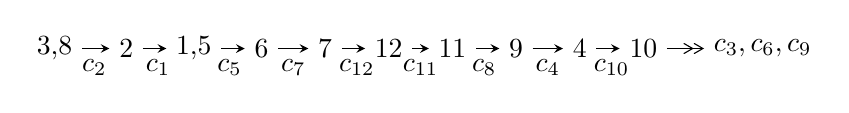
\begin{tikzpicture}[x=23pt, y=7pt]
	% node
	\node (A0) at (-1/8, 0) {3,8};
	\node (A1) at (1, 0) {2};
	\node (A2) at (33/16, 0) {1,5};
	\node (A3) at (25/8, 0) {6};
	\node (A4) at (33/8, 0) {7};
	\node (A5) at (41/8, 0) {12};
	\node (A6) at (49/8, 0) {11};
	\node (A7) at (57/8, 0) {9};
	\node (A8) at (65/8, 0) {4};
	\node (A9) at (73/8, 0) {10};
	\node (C1) at (1/2, -1) {$c_{2}$};
	\node (C2) at (3/2, -1) {$c_{1}$};
	\node (C3) at (21/8, -1) {$c_{5}$};
	\node (C4) at (29/8, -1) {$c_{7}$};
	\node (C5) at (37/8, -1) {$c_{12}$};
	\node (C6) at (45/8, -1) {$c_{11}$};
	\node (C7) at (53/8, -1) {$c_{8}$};
	\node (C8) at (61/8, -1) {$c_{4}$};
	\node (C9) at (69/8, -1) {$c_{10}$};
	\node (A10) at (11, 0) {$c_{3},c_{6},c_{9}$};

	% edge
	\draw[->,>=stealth]	
	(A0) edge (A1) (A1) edge (A2) (A2) edge (A3) (A3) edge (A4) (A4) edge (A5) (A5) edge (A6) (A6) edge (A7) (A7) edge (A8) (A8) edge (A9) ;
	\draw[->>,>={angle 60}]	
	(A9) edge (A10);
\end{tikzpicture} \\ 

\end{tabular} \\

\footnotetext{
The image of knot diagram is generated by the software ``\textbf{Draw programme}" developed by Andrew Bartholomew(\url{http://www.layer8.co.uk/maths/draw/index.htm\#Running-draw}), where we modified some parts for our purpose(\url{https://github.com/CATsTAILs/LinksPainter}).
}\phantom \\ \newline 
\centering \textbf{Ideals for irreducible components\footnotemark of $X_{\text{par}}$} 
 
\begin{align*}
I^u_{1}&=\langle 
-7.95566\times10^{237} u^{100}-6.62307\times10^{237} u^{99}+\cdots+4.78420\times10^{238} b-4.22616\times10^{240},\\
\phantom{I^u_{1}}&\phantom{= \langle  }-5.09303\times10^{240} u^{100}-6.43646\times10^{240} u^{99}+\cdots+1.00947\times10^{241} a-1.17880\times10^{243},\\
\phantom{I^u_{1}}&\phantom{= \langle  }u^{101}-29 u^{99}+\cdots-366 u-211\rangle \\
I^u_{2}&=\langle 
-6594748663 u^{31}+11676405243 u^{30}+\cdots+304614406 b-9241004294,\\
\phantom{I^u_{2}}&\phantom{= \langle  }9719505347 u^{31}-16695825813 u^{30}+\cdots+304614406 a+11648772074,\;u^{32}- u^{31}+\cdots-3 u+1\rangle \\
\\
\end{align*}
\raggedright * 2 irreducible components of $\dim_{\mathbb{C}}=0$, with total 133 representations.\\
\footnotetext{All coefficients of polynomials are rational numbers. But the coefficients are sometimes approximated in decimal forms when there is not enough margin.}
\newpage
\renewcommand{\arraystretch}{1}
\centering \section*{I. $I^u_{1}= \langle -7.96\times10^{237} u^{100}-6.62\times10^{237} u^{99}+\cdots+4.78\times10^{238} b-4.23\times10^{240},\;-5.09\times10^{240} u^{100}-6.44\times10^{240} u^{99}+\cdots+1.01\times10^{241} a-1.18\times10^{243},\;u^{101}-29 u^{99}+\cdots-366 u-211 \rangle$}
\flushleft \textbf{(i) Arc colorings}\\
\begin{tabular}{m{7pt} m{180pt} m{7pt} m{180pt} }
\flushright $a_{3}=$&$\begin{pmatrix}1\\0\end{pmatrix}$ \\
\flushright $a_{8}=$&$\begin{pmatrix}0\\u\end{pmatrix}$ \\
\flushright $a_{2}=$&$\begin{pmatrix}1\\- u^2\end{pmatrix}$ \\
\flushright $a_{1}=$&$\begin{pmatrix}- u^2+1\\- u^2\end{pmatrix}$ \\
\flushright $a_{5}=$&$\begin{pmatrix}0.504526 u^{100}+0.637610 u^{99}+\cdots+220.410 u+116.774\\0.166290 u^{100}+0.138436 u^{99}+\cdots+298.648 u+88.3358\end{pmatrix}$ \\
\flushright $a_{6}=$&$\begin{pmatrix}0.719768 u^{100}+0.816275 u^{99}+\cdots+396.415 u+177.901\\-0.314263 u^{100}-0.311027 u^{99}+\cdots-78.0601 u-44.1993\end{pmatrix}$ \\
\flushright $a_{7}=$&$\begin{pmatrix}u\\- u^3+u\end{pmatrix}$ \\
\flushright $a_{12}=$&$\begin{pmatrix}0.0646741 u^{100}+0.102419 u^{99}+\cdots-5.30493 u+10.0598\\0.709533 u^{100}+0.284808 u^{99}+\cdots+376.424 u+77.2488\end{pmatrix}$ \\
\flushright $a_{11}=$&$\begin{pmatrix}0.0646741 u^{100}+0.102419 u^{99}+\cdots-5.30493 u+10.0598\\0.560079 u^{100}+0.146742 u^{99}+\cdots+325.292 u+55.6384\end{pmatrix}$ \\
\flushright $a_{9}=$&$\begin{pmatrix}0.574178 u^{100}+0.482635 u^{99}+\cdots+367.785 u+130.977\\-0.0616652 u^{100}-0.285923 u^{99}+\cdots-131.623 u-77.5243\end{pmatrix}$ \\
\flushright $a_{4}=$&$\begin{pmatrix}1.02386 u^{100}+0.779755 u^{99}+\cdots+593.132 u+198.503\\-0.120196 u^{100}-0.169073 u^{99}+\cdots-85.7088 u-33.7270\end{pmatrix}$ \\
\flushright $a_{10}=$&$\begin{pmatrix}0.716347 u^{100}+0.710368 u^{99}+\cdots+544.466 u+211.942\\0.0100619 u^{100}-0.152637 u^{99}+\cdots-68.2902 u-44.6114\end{pmatrix}$\\&\end{tabular}
\flushleft \textbf{(ii) Obstruction class $= -1$}\\~\\
\flushleft \textbf{(iii) Cusp Shapes $= -4.64685 u^{100}-3.26032 u^{99}+\cdots-3712.21 u-1141.11$}\\~\\
\newpage\renewcommand{\arraystretch}{1}
\flushleft \textbf{(iv) u-Polynomials at the component}\newline \\
\begin{tabular}{m{50pt}|m{274pt}}
Crossings & \hspace{64pt}u-Polynomials at each crossing \\
\hline $$\begin{aligned}c_{1}\end{aligned}$$&$\begin{aligned}
&u^{101}+58 u^{100}+\cdots+943774 u+44521
\end{aligned}$\\
\hline $$\begin{aligned}c_{2},c_{7}\end{aligned}$$&$\begin{aligned}
&u^{101}-29 u^{99}+\cdots-366 u-211
\end{aligned}$\\
\hline $$\begin{aligned}c_{3}\end{aligned}$$&$\begin{aligned}
&u^{101}-2 u^{100}+\cdots-97 u+7
\end{aligned}$\\
\hline $$\begin{aligned}c_{4}\end{aligned}$$&$\begin{aligned}
&u^{101}+23 u^{99}+\cdots+750579 u+306659
\end{aligned}$\\
\hline $$\begin{aligned}c_{5},c_{12}\end{aligned}$$&$\begin{aligned}
&u^{101}-16 u^{99}+\cdots-953 u-133
\end{aligned}$\\
\hline $$\begin{aligned}c_{6}\end{aligned}$$&$\begin{aligned}
&u^{101}- u^{100}+\cdots+227 u-23
\end{aligned}$\\
\hline $$\begin{aligned}c_{8},c_{11}\end{aligned}$$&$\begin{aligned}
&u^{101}+15 u^{100}+\cdots+3501095 u+215671
\end{aligned}$\\
\hline $$\begin{aligned}c_{9}\end{aligned}$$&$\begin{aligned}
&u^{101}-7 u^{100}+\cdots-1316600 u+92575
\end{aligned}$\\
\hline $$\begin{aligned}c_{10}\end{aligned}$$&$\begin{aligned}
&u^{101}-3 u^{100}+\cdots-790 u-83
\end{aligned}$\\
\hline
\end{tabular}\\~\\
\newpage\renewcommand{\arraystretch}{1}
\flushleft \textbf{(v) Riley Polynomials at the component}\newline \\
\begin{tabular}{m{50pt}|m{274pt}}
Crossings & \hspace{64pt}Riley Polynomials at each crossing \\
\hline $$\begin{aligned}c_{1}\end{aligned}$$&$\begin{aligned}
&y^{101}-14 y^{100}+\cdots+27975815430 y-1982119441
\end{aligned}$\\
\hline $$\begin{aligned}c_{2},c_{7}\end{aligned}$$&$\begin{aligned}
&y^{101}-58 y^{100}+\cdots+943774 y-44521
\end{aligned}$\\
\hline $$\begin{aligned}c_{3}\end{aligned}$$&$\begin{aligned}
&y^{101}-10 y^{100}+\cdots+155 y-49
\end{aligned}$\\
\hline $$\begin{aligned}c_{4}\end{aligned}$$&$\begin{aligned}
&y^{101}+46 y^{100}+\cdots-3797359557157 y-94039742281
\end{aligned}$\\
\hline $$\begin{aligned}c_{5},c_{12}\end{aligned}$$&$\begin{aligned}
&y^{101}-32 y^{100}+\cdots+823621 y-17689
\end{aligned}$\\
\hline $$\begin{aligned}c_{6}\end{aligned}$$&$\begin{aligned}
&y^{101}-9 y^{100}+\cdots+23423 y-529
\end{aligned}$\\
\hline $$\begin{aligned}c_{8},c_{11}\end{aligned}$$&$\begin{aligned}
&y^{101}-93 y^{100}+\cdots+1171525903947 y-46513980241
\end{aligned}$\\
\hline $$\begin{aligned}c_{9}\end{aligned}$$&$\begin{aligned}
&y^{101}-45 y^{100}+\cdots+570114040500 y-8570130625
\end{aligned}$\\
\hline $$\begin{aligned}c_{10}\end{aligned}$$&$\begin{aligned}
&y^{101}+11 y^{100}+\cdots-196936 y-6889
\end{aligned}$\\
\hline
\end{tabular}\\~\\
\newpage\flushleft \textbf{(vi) Complex Volumes and Cusp Shapes}
$$\begin{array}{c|c|c}  
\text{Solutions to }I^u_{1}& \I (\text{vol} + \sqrt{-1}CS) & \text{Cusp shape}\\
 \hline 
\begin{aligned}
u &= \phantom{-}0.820034 + 0.585292 I \\
a &= \phantom{-}0.033824 - 0.300405 I \\
b &= -0.94355 - 1.29230 I\end{aligned}
 & \phantom{-}4.33943 + 1.14415 I & \phantom{-0.000000 } 0 \\ \hline\begin{aligned}
u &= \phantom{-}0.820034 - 0.585292 I \\
a &= \phantom{-}0.033824 + 0.300405 I \\
b &= -0.94355 + 1.29230 I\end{aligned}
 & \phantom{-}4.33943 - 1.14415 I & \phantom{-0.000000 } 0 \\ \hline\begin{aligned}
u &= \phantom{-}0.985457 + 0.104624 I \\
a &= \phantom{-}0.037446 - 0.669943 I \\
b &= \phantom{-}0.726416 + 0.509050 I\end{aligned}
 & -3.62929 - 2.83489 I & \phantom{-0.000000 } 0 \\ \hline\begin{aligned}
u &= \phantom{-}0.985457 - 0.104624 I \\
a &= \phantom{-}0.037446 + 0.669943 I \\
b &= \phantom{-}0.726416 - 0.509050 I\end{aligned}
 & -3.62929 + 2.83489 I & \phantom{-0.000000 } 0 \\ \hline\begin{aligned}
u &= -0.530981 + 0.810422 I \\
a &= \phantom{-}1.61271 - 1.19757 I \\
b &= \phantom{-}0.532324 - 0.580869 I\end{aligned}
 & -2.63257 + 3.84014 I & \phantom{-0.000000 } 0 \\ \hline\begin{aligned}
u &= -0.530981 - 0.810422 I \\
a &= \phantom{-}1.61271 + 1.19757 I \\
b &= \phantom{-}0.532324 + 0.580869 I\end{aligned}
 & -2.63257 - 3.84014 I & \phantom{-0.000000 } 0 \\ \hline\begin{aligned}
u &= \phantom{-}1.027270 + 0.217643 I \\
a &= -0.340119 - 1.308040 I \\
b &= \phantom{-}0.243063 - 1.221120 I\end{aligned}
 & -7.61850 - 0.65923 I & \phantom{-0.000000 } 0 \\ \hline\begin{aligned}
u &= \phantom{-}1.027270 - 0.217643 I \\
a &= -0.340119 + 1.308040 I \\
b &= \phantom{-}0.243063 + 1.221120 I\end{aligned}
 & -7.61850 + 0.65923 I & \phantom{-0.000000 } 0 \\ \hline\begin{aligned}
u &= -0.112192 + 0.938796 I \\
a &= \phantom{-}1.95188 - 0.30689 I \\
b &= \phantom{-}0.468388 + 0.284137 I\end{aligned}
 & -1.67442 - 1.04305 I & \phantom{-0.000000 } 0 \\ \hline\begin{aligned}
u &= -0.112192 - 0.938796 I \\
a &= \phantom{-}1.95188 + 0.30689 I \\
b &= \phantom{-}0.468388 - 0.284137 I\end{aligned}
 & -1.67442 + 1.04305 I & \phantom{-0.000000 } 0\\
 \hline 
 \end{array}$$\newpage$$\begin{array}{c|c|c}  
\text{Solutions to }I^u_{1}& \I (\text{vol} + \sqrt{-1}CS) & \text{Cusp shape}\\
 \hline 
\begin{aligned}
u &= \phantom{-}0.172731 + 1.067630 I \\
a &= \phantom{-}1.47812 - 0.48759 I \\
b &= \phantom{-}0.295965 - 0.883833 I\end{aligned}
 & -0.38324 + 3.98606 I & \phantom{-0.000000 } 0 \\ \hline\begin{aligned}
u &= \phantom{-}0.172731 - 1.067630 I \\
a &= \phantom{-}1.47812 + 0.48759 I \\
b &= \phantom{-}0.295965 + 0.883833 I\end{aligned}
 & -0.38324 - 3.98606 I & \phantom{-0.000000 } 0 \\ \hline\begin{aligned}
u &= -0.422357 + 0.996136 I \\
a &= \phantom{-}1.88932 + 0.35696 I \\
b &= \phantom{-}0.689307 + 1.005280 I\end{aligned}
 & -2.01850 - 3.05243 I & \phantom{-0.000000 } 0 \\ \hline\begin{aligned}
u &= -0.422357 - 0.996136 I \\
a &= \phantom{-}1.88932 - 0.35696 I \\
b &= \phantom{-}0.689307 - 1.005280 I\end{aligned}
 & -2.01850 + 3.05243 I & \phantom{-0.000000 } 0 \\ \hline\begin{aligned}
u &= -0.832349 + 0.372279 I \\
a &= -0.139598 + 1.207060 I \\
b &= -0.0679636 - 0.0471394 I\end{aligned}
 & \phantom{-}1.34976 - 0.66315 I & \phantom{-0.000000 } 0 \\ \hline\begin{aligned}
u &= -0.832349 - 0.372279 I \\
a &= -0.139598 - 1.207060 I \\
b &= -0.0679636 + 0.0471394 I\end{aligned}
 & \phantom{-}1.34976 + 0.66315 I & \phantom{-0.000000 } 0 \\ \hline\begin{aligned}
u &= -0.656254 + 0.632742 I \\
a &= \phantom{-}0.564801 - 1.036380 I \\
b &= \phantom{-}0.962520 - 0.528825 I\end{aligned}
 & -0.33221 + 2.15160 I & \phantom{-0.000000 } 0 \\ \hline\begin{aligned}
u &= -0.656254 - 0.632742 I \\
a &= \phantom{-}0.564801 + 1.036380 I \\
b &= \phantom{-}0.962520 + 0.528825 I\end{aligned}
 & -0.33221 - 2.15160 I & \phantom{-0.000000 } 0 \\ \hline\begin{aligned}
u &= -0.421401 + 0.800169 I \\
a &= -1.125030 + 0.132865 I \\
b &= -0.293273 - 0.851923 I\end{aligned}
 & -2.71761 - 1.32653 I & \phantom{-0.000000 } 0 \\ \hline\begin{aligned}
u &= -0.421401 - 0.800169 I \\
a &= -1.125030 - 0.132865 I \\
b &= -0.293273 + 0.851923 I\end{aligned}
 & -2.71761 + 1.32653 I & \phantom{-0.000000 } 0\\
 \hline 
 \end{array}$$\newpage$$\begin{array}{c|c|c}  
\text{Solutions to }I^u_{1}& \I (\text{vol} + \sqrt{-1}CS) & \text{Cusp shape}\\
 \hline 
\begin{aligned}
u &= \phantom{-}0.259609 + 1.067610 I \\
a &= -1.72155 + 0.32265 I \\
b &= -0.466377 + 0.881217 I\end{aligned}
 & -1.92144 + 12.29610 I & \phantom{-0.000000 } 0 \\ \hline\begin{aligned}
u &= \phantom{-}0.259609 - 1.067610 I \\
a &= -1.72155 - 0.32265 I \\
b &= -0.466377 - 0.881217 I\end{aligned}
 & -1.92144 - 12.29610 I & \phantom{-0.000000 } 0 \\ \hline\begin{aligned}
u &= -0.723110 + 0.827949 I \\
a &= \phantom{-}0.84434 + 1.80493 I \\
b &= -0.38782 + 1.81403 I\end{aligned}
 & \phantom{-}2.61470 - 2.35298 I & \phantom{-0.000000 } 0 \\ \hline\begin{aligned}
u &= -0.723110 - 0.827949 I \\
a &= \phantom{-}0.84434 - 1.80493 I \\
b &= -0.38782 - 1.81403 I\end{aligned}
 & \phantom{-}2.61470 + 2.35298 I & \phantom{-0.000000 } 0 \\ \hline\begin{aligned}
u &= -0.947967 + 0.574342 I \\
a &= \phantom{-}0.878995 - 0.261408 I \\
b &= \phantom{-}0.142593 + 0.500799 I\end{aligned}
 & -1.15276 + 2.52280 I & \phantom{-0.000000 } 0 \\ \hline\begin{aligned}
u &= -0.947967 - 0.574342 I \\
a &= \phantom{-}0.878995 + 0.261408 I \\
b &= \phantom{-}0.142593 - 0.500799 I\end{aligned}
 & -1.15276 - 2.52280 I & \phantom{-0.000000 } 0 \\ \hline\begin{aligned}
u &= -0.825651 + 0.325227 I \\
a &= -1.03139 + 1.08118 I \\
b &= -1.96412 + 0.68654 I\end{aligned}
 & \phantom{-}1.46496 + 3.76761 I & \phantom{-0.000000 } 0 \\ \hline\begin{aligned}
u &= -0.825651 - 0.325227 I \\
a &= -1.03139 - 1.08118 I \\
b &= -1.96412 - 0.68654 I\end{aligned}
 & \phantom{-}1.46496 - 3.76761 I & \phantom{-0.000000 } 0 \\ \hline\begin{aligned}
u &= \phantom{-}1.037520 + 0.423630 I \\
a &= -0.655068 - 0.350769 I \\
b &= -0.390864 + 1.168550 I\end{aligned}
 & \phantom{-}1.02564 - 5.30362 I & \phantom{-0.000000 } 0 \\ \hline\begin{aligned}
u &= \phantom{-}1.037520 - 0.423630 I \\
a &= -0.655068 + 0.350769 I \\
b &= -0.390864 - 1.168550 I\end{aligned}
 & \phantom{-}1.02564 + 5.30362 I & \phantom{-0.000000 } 0\\
 \hline 
 \end{array}$$\newpage$$\begin{array}{c|c|c}  
\text{Solutions to }I^u_{1}& \I (\text{vol} + \sqrt{-1}CS) & \text{Cusp shape}\\
 \hline 
\begin{aligned}
u &= -1.091290 + 0.326589 I \\
a &= -0.125661 + 0.458687 I \\
b &= -0.98139 + 2.35676 I\end{aligned}
 & \phantom{-}1.78195 + 6.72216 I & \phantom{-0.000000 } 0 \\ \hline\begin{aligned}
u &= -1.091290 - 0.326589 I \\
a &= -0.125661 - 0.458687 I \\
b &= -0.98139 - 2.35676 I\end{aligned}
 & \phantom{-}1.78195 - 6.72216 I & \phantom{-0.000000 } 0 \\ \hline\begin{aligned}
u &= \phantom{-}0.715518 + 0.470453 I \\
a &= -0.146982 - 0.233324 I \\
b &= \phantom{-}1.19859 + 0.91932 I\end{aligned}
 & \phantom{-}4.69000 - 5.44399 I & \phantom{-0.000000 } 0 \\ \hline\begin{aligned}
u &= \phantom{-}0.715518 - 0.470453 I \\
a &= -0.146982 + 0.233324 I \\
b &= \phantom{-}1.19859 - 0.91932 I\end{aligned}
 & \phantom{-}4.69000 + 5.44399 I & \phantom{-0.000000 } 0 \\ \hline\begin{aligned}
u &= \phantom{-}1.105060 + 0.348432 I \\
a &= -0.429969 - 1.131870 I \\
b &= -0.29685 - 1.62962 I\end{aligned}
 & -5.52117 + 1.02862 I & \phantom{-0.000000 } 0 \\ \hline\begin{aligned}
u &= \phantom{-}1.105060 - 0.348432 I \\
a &= -0.429969 + 1.131870 I \\
b &= -0.29685 + 1.62962 I\end{aligned}
 & -5.52117 - 1.02862 I & \phantom{-0.000000 } 0 \\ \hline\begin{aligned}
u &= \phantom{-}0.834281 + 0.073903 I \\
a &= -0.085148 - 1.349500 I \\
b &= \phantom{-}0.742747 + 0.274742 I\end{aligned}
 & -3.70589 - 2.85195 I & \phantom{-0.000000 } 0 \\ \hline\begin{aligned}
u &= \phantom{-}0.834281 - 0.073903 I \\
a &= -0.085148 + 1.349500 I \\
b &= \phantom{-}0.742747 - 0.274742 I\end{aligned}
 & -3.70589 + 2.85195 I & \phantom{-0.000000 } 0 \\ \hline\begin{aligned}
u &= \phantom{-}1.168720 + 0.132657 I \\
a &= \phantom{-}0.374634 + 1.230770 I \\
b &= \phantom{-}0.446630 + 1.106190 I\end{aligned}
 & -8.14969 + 0.29983 I & \phantom{-0.000000 } 0 \\ \hline\begin{aligned}
u &= \phantom{-}1.168720 - 0.132657 I \\
a &= \phantom{-}0.374634 - 1.230770 I \\
b &= \phantom{-}0.446630 - 1.106190 I\end{aligned}
 & -8.14969 - 0.29983 I & \phantom{-0.000000 } 0\\
 \hline 
 \end{array}$$\newpage$$\begin{array}{c|c|c}  
\text{Solutions to }I^u_{1}& \I (\text{vol} + \sqrt{-1}CS) & \text{Cusp shape}\\
 \hline 
\begin{aligned}
u &= \phantom{-}1.057890 + 0.529949 I \\
a &= -0.549762 + 0.270888 I \\
b &= \phantom{-}0.32388 + 1.47416 I\end{aligned}
 & \phantom{-}0.69986 - 5.52879 I & \phantom{-0.000000 } 0 \\ \hline\begin{aligned}
u &= \phantom{-}1.057890 - 0.529949 I \\
a &= -0.549762 - 0.270888 I \\
b &= \phantom{-}0.32388 - 1.47416 I\end{aligned}
 & \phantom{-}0.69986 + 5.52879 I & \phantom{-0.000000 } 0 \\ \hline\begin{aligned}
u &= \phantom{-}1.133440 + 0.362308 I \\
a &= \phantom{-}0.37569 + 1.43089 I \\
b &= \phantom{-}2.68251 + 2.44321 I\end{aligned}
 & -6.79023 - 6.46863 I & \phantom{-0.000000 } 0 \\ \hline\begin{aligned}
u &= \phantom{-}1.133440 - 0.362308 I \\
a &= \phantom{-}0.37569 - 1.43089 I \\
b &= \phantom{-}2.68251 - 2.44321 I\end{aligned}
 & -6.79023 + 6.46863 I & \phantom{-0.000000 } 0 \\ \hline\begin{aligned}
u &= \phantom{-}0.774969 + 0.908000 I \\
a &= \phantom{-}0.847818 - 0.971440 I \\
b &= -0.253631 - 1.291530 I\end{aligned}
 & \phantom{-}4.25675 - 0.06797 I & \phantom{-0.000000 } 0 \\ \hline\begin{aligned}
u &= \phantom{-}0.774969 - 0.908000 I \\
a &= \phantom{-}0.847818 + 0.971440 I \\
b &= -0.253631 + 1.291530 I\end{aligned}
 & \phantom{-}4.25675 + 0.06797 I & \phantom{-0.000000 } 0 \\ \hline\begin{aligned}
u &= -1.165960 + 0.275055 I \\
a &= \phantom{-}0.456960 + 0.048402 I \\
b &= \phantom{-}0.603489 - 0.827587 I\end{aligned}
 & -1.65982 + 1.25712 I & \phantom{-0.000000 } 0 \\ \hline\begin{aligned}
u &= -1.165960 - 0.275055 I \\
a &= \phantom{-}0.456960 - 0.048402 I \\
b &= \phantom{-}0.603489 + 0.827587 I\end{aligned}
 & -1.65982 - 1.25712 I & \phantom{-0.000000 } 0 \\ \hline\begin{aligned}
u &= \phantom{-}0.598387 + 0.502597 I \\
a &= \phantom{-}0.32061 - 1.55924 I \\
b &= -1.45875 - 1.20083 I\end{aligned}
 & \phantom{-}2.45000 + 1.47696 I & -2.21815 + 0. I\phantom{ +0.000000I} \\ \hline\begin{aligned}
u &= \phantom{-}0.598387 - 0.502597 I \\
a &= \phantom{-}0.32061 + 1.55924 I \\
b &= -1.45875 + 1.20083 I\end{aligned}
 & \phantom{-}2.45000 - 1.47696 I & -2.21815 + 0. I\phantom{ +0.000000I}\\
 \hline 
 \end{array}$$\newpage$$\begin{array}{c|c|c}  
\text{Solutions to }I^u_{1}& \I (\text{vol} + \sqrt{-1}CS) & \text{Cusp shape}\\
 \hline 
\begin{aligned}
u &= -0.781170\phantom{ +0.000000I} \\
a &= -0.660008\phantom{ +0.000000I} \\
b &= -2.65405\phantom{ +0.000000I}\end{aligned}
 & \phantom{-}0.526391\phantom{ +0.000000I} & -12.4510\phantom{ +0.000000I} \\ \hline\begin{aligned}
u &= \phantom{-}1.165080 + 0.391120 I \\
a &= -0.554888 - 1.188060 I \\
b &= -2.46665 - 2.02558 I\end{aligned}
 & -7.73546 + 1.92109 I & \phantom{-0.000000 } 0 \\ \hline\begin{aligned}
u &= \phantom{-}1.165080 - 0.391120 I \\
a &= -0.554888 + 1.188060 I \\
b &= -2.46665 + 2.02558 I\end{aligned}
 & -7.73546 - 1.92109 I & \phantom{-0.000000 } 0 \\ \hline\begin{aligned}
u &= -1.113090 + 0.539386 I \\
a &= \phantom{-}0.412358 - 0.117499 I \\
b &= \phantom{-}0.398639 + 0.659751 I\end{aligned}
 & \phantom{-}0.260818 - 0.400392 I & \phantom{-0.000000 } 0 \\ \hline\begin{aligned}
u &= -1.113090 - 0.539386 I \\
a &= \phantom{-}0.412358 + 0.117499 I \\
b &= \phantom{-}0.398639 - 0.659751 I\end{aligned}
 & \phantom{-}0.260818 + 0.400392 I & \phantom{-0.000000 } 0 \\ \hline\begin{aligned}
u &= -0.297259 + 0.702085 I \\
a &= -1.71072 + 0.42820 I \\
b &= -0.086831 - 0.815638 I\end{aligned}
 & -1.72276 - 3.92826 I & -4.92577 + 8.41157 I \\ \hline\begin{aligned}
u &= -0.297259 - 0.702085 I \\
a &= -1.71072 - 0.42820 I \\
b &= -0.086831 + 0.815638 I\end{aligned}
 & -1.72276 + 3.92826 I & -4.92577 - 8.41157 I \\ \hline\begin{aligned}
u &= -1.004280 + 0.734721 I \\
a &= -1.49398 - 1.38619 I \\
b &= \phantom{-}0.06660 - 2.24573 I\end{aligned}
 & \phantom{-}1.74154 + 8.20625 I & \phantom{-0.000000 } 0 \\ \hline\begin{aligned}
u &= -1.004280 - 0.734721 I \\
a &= -1.49398 + 1.38619 I \\
b &= \phantom{-}0.06660 + 2.24573 I\end{aligned}
 & \phantom{-}1.74154 - 8.20625 I & \phantom{-0.000000 } 0 \\ \hline\begin{aligned}
u &= \phantom{-}0.387915 + 0.646900 I \\
a &= \phantom{-}0.341745 - 0.685172 I \\
b &= -0.754171 - 0.784952 I\end{aligned}
 & \phantom{-}2.62272 + 0.97071 I & \phantom{-}1.85950 - 0.63323 I\\
 \hline 
 \end{array}$$\newpage$$\begin{array}{c|c|c}  
\text{Solutions to }I^u_{1}& \I (\text{vol} + \sqrt{-1}CS) & \text{Cusp shape}\\
 \hline 
\begin{aligned}
u &= \phantom{-}0.387915 - 0.646900 I \\
a &= \phantom{-}0.341745 + 0.685172 I \\
b &= -0.754171 + 0.784952 I\end{aligned}
 & \phantom{-}2.62272 - 0.97071 I & \phantom{-}1.85950 + 0.63323 I \\ \hline\begin{aligned}
u &= -1.128540 + 0.535413 I \\
a &= -0.315092 + 1.093540 I \\
b &= -1.92869 + 1.96354 I\end{aligned}
 & -4.14830 + 8.67493 I & \phantom{-0.000000 } 0 \\ \hline\begin{aligned}
u &= -1.128540 - 0.535413 I \\
a &= -0.315092 - 1.093540 I \\
b &= -1.92869 - 1.96354 I\end{aligned}
 & -4.14830 - 8.67493 I & \phantom{-0.000000 } 0 \\ \hline\begin{aligned}
u &= -0.749799\phantom{ +0.000000I} \\
a &= \phantom{-}0.510552\phantom{ +0.000000I} \\
b &= \phantom{-}0.219990\phantom{ +0.000000I}\end{aligned}
 & -1.51667\phantom{ +0.000000I} & -5.25440\phantom{ +0.000000I} \\ \hline\begin{aligned}
u &= -0.192427 + 0.718269 I \\
a &= -2.15738 + 0.48060 I \\
b &= -0.342576 + 0.575969 I\end{aligned}
 & -4.01739 - 5.53614 I & -4.00000 + 3.69769 I \\ \hline\begin{aligned}
u &= -0.192427 - 0.718269 I \\
a &= -2.15738 - 0.48060 I \\
b &= -0.342576 - 0.575969 I\end{aligned}
 & -4.01739 + 5.53614 I & -4.00000 - 3.69769 I \\ \hline\begin{aligned}
u &= -1.117260 + 0.604980 I \\
a &= -0.121036 + 1.042240 I \\
b &= -1.67025 + 1.58440 I\end{aligned}
 & -4.80170 + 6.61061 I & \phantom{-0.000000 } 0 \\ \hline\begin{aligned}
u &= -1.117260 - 0.604980 I \\
a &= -0.121036 - 1.042240 I \\
b &= -1.67025 - 1.58440 I\end{aligned}
 & -4.80170 - 6.61061 I & \phantom{-0.000000 } 0 \\ \hline\begin{aligned}
u &= -1.165570 + 0.513406 I \\
a &= -0.449779 + 1.143800 I \\
b &= -0.229696 + 1.391280 I\end{aligned}
 & -6.84123 + 10.22070 I & \phantom{-0.000000 } 0 \\ \hline\begin{aligned}
u &= -1.165570 - 0.513406 I \\
a &= -0.449779 - 1.143800 I \\
b &= -0.229696 - 1.391280 I\end{aligned}
 & -6.84123 - 10.22070 I & \phantom{-0.000000 } 0\\
 \hline 
 \end{array}$$\newpage$$\begin{array}{c|c|c}  
\text{Solutions to }I^u_{1}& \I (\text{vol} + \sqrt{-1}CS) & \text{Cusp shape}\\
 \hline 
\begin{aligned}
u &= \phantom{-}1.211150 + 0.458943 I \\
a &= -0.156975 + 0.229898 I \\
b &= -0.571082 - 0.377330 I\end{aligned}
 & -0.47114 - 9.20279 I & \phantom{-0.000000 } 0 \\ \hline\begin{aligned}
u &= \phantom{-}1.211150 - 0.458943 I \\
a &= -0.156975 - 0.229898 I \\
b &= -0.571082 + 0.377330 I\end{aligned}
 & -0.47114 + 9.20279 I & \phantom{-0.000000 } 0 \\ \hline\begin{aligned}
u &= -0.051611 + 0.697056 I \\
a &= \phantom{-}0.410927 - 0.410638 I \\
b &= \phantom{-}0.784635 + 0.092928 I\end{aligned}
 & \phantom{-}3.06555 + 4.91909 I & \phantom{-}0.44965 - 7.59677 I \\ \hline\begin{aligned}
u &= -0.051611 - 0.697056 I \\
a &= \phantom{-}0.410927 + 0.410638 I \\
b &= \phantom{-}0.784635 - 0.092928 I\end{aligned}
 & \phantom{-}3.06555 - 4.91909 I & \phantom{-}0.44965 + 7.59677 I \\ \hline\begin{aligned}
u &= \phantom{-}1.292030 + 0.181188 I \\
a &= \phantom{-}0.157375 + 0.926748 I \\
b &= \phantom{-}0.587242 + 1.239310 I\end{aligned}
 & -6.11471 - 3.27045 I & \phantom{-0.000000 } 0 \\ \hline\begin{aligned}
u &= \phantom{-}1.292030 - 0.181188 I \\
a &= \phantom{-}0.157375 - 0.926748 I \\
b &= \phantom{-}0.587242 - 1.239310 I\end{aligned}
 & -6.11471 + 3.27045 I & \phantom{-0.000000 } 0 \\ \hline\begin{aligned}
u &= \phantom{-}1.264860 + 0.336878 I \\
a &= \phantom{-}0.299011 + 1.080750 I \\
b &= \phantom{-}0.47582 + 1.36586 I\end{aligned}
 & -6.25089 - 3.34515 I & \phantom{-0.000000 } 0 \\ \hline\begin{aligned}
u &= \phantom{-}1.264860 - 0.336878 I \\
a &= \phantom{-}0.299011 - 1.080750 I \\
b &= \phantom{-}0.47582 - 1.36586 I\end{aligned}
 & -6.25089 + 3.34515 I & \phantom{-0.000000 } 0 \\ \hline\begin{aligned}
u &= \phantom{-}0.985067 + 0.899162 I \\
a &= -0.449526 + 1.155670 I \\
b &= \phantom{-}0.42203 + 1.54482 I\end{aligned}
 & \phantom{-}3.65832 - 6.49471 I & \phantom{-0.000000 } 0 \\ \hline\begin{aligned}
u &= \phantom{-}0.985067 - 0.899162 I \\
a &= -0.449526 - 1.155670 I \\
b &= \phantom{-}0.42203 - 1.54482 I\end{aligned}
 & \phantom{-}3.65832 + 6.49471 I & \phantom{-0.000000 } 0\\
 \hline 
 \end{array}$$\newpage$$\begin{array}{c|c|c}  
\text{Solutions to }I^u_{1}& \I (\text{vol} + \sqrt{-1}CS) & \text{Cusp shape}\\
 \hline 
\begin{aligned}
u &= -1.237570 + 0.506251 I \\
a &= \phantom{-}0.660880 - 1.087730 I \\
b &= \phantom{-}1.90594 - 1.83014 I\end{aligned}
 & -5.17592 + 6.17586 I & \phantom{-0.000000 } 0 \\ \hline\begin{aligned}
u &= -1.237570 - 0.506251 I \\
a &= \phantom{-}0.660880 + 1.087730 I \\
b &= \phantom{-}1.90594 + 1.83014 I\end{aligned}
 & -5.17592 - 6.17586 I & \phantom{-0.000000 } 0 \\ \hline\begin{aligned}
u &= \phantom{-}0.649004 + 0.074296 I \\
a &= \phantom{-}0.51392 + 2.77828 I \\
b &= \phantom{-}0.27129 - 2.39289 I\end{aligned}
 & -4.46140 + 4.15869 I & \phantom{-}3.67911 - 0.78240 I \\ \hline\begin{aligned}
u &= \phantom{-}0.649004 - 0.074296 I \\
a &= \phantom{-}0.51392 - 2.77828 I \\
b &= \phantom{-}0.27129 + 2.39289 I\end{aligned}
 & -4.46140 - 4.15869 I & \phantom{-}3.67911 + 0.78240 I \\ \hline\begin{aligned}
u &= -1.196790 + 0.651190 I \\
a &= \phantom{-}0.19788 - 1.58630 I \\
b &= \phantom{-}1.65935 - 2.17229 I\end{aligned}
 & -4.47841 + 9.04243 I & \phantom{-0.000000 } 0 \\ \hline\begin{aligned}
u &= -1.196790 - 0.651190 I \\
a &= \phantom{-}0.19788 + 1.58630 I \\
b &= \phantom{-}1.65935 + 2.17229 I\end{aligned}
 & -4.47841 - 9.04243 I & \phantom{-0.000000 } 0 \\ \hline\begin{aligned}
u &= -1.243550 + 0.563865 I \\
a &= \phantom{-}0.742729 - 0.977181 I \\
b &= \phantom{-}0.526850 - 1.039350 I\end{aligned}
 & -5.08145 + 1.93675 I & \phantom{-0.000000 } 0 \\ \hline\begin{aligned}
u &= -1.243550 - 0.563865 I \\
a &= \phantom{-}0.742729 + 0.977181 I \\
b &= \phantom{-}0.526850 + 1.039350 I\end{aligned}
 & -5.08145 - 1.93675 I & \phantom{-0.000000 } 0 \\ \hline\begin{aligned}
u &= -0.603686 + 0.144992 I \\
a &= -0.391023 + 0.681439 I \\
b &= \phantom{-}1.84033 - 1.17193 I\end{aligned}
 & \phantom{-}3.67321 - 4.24686 I & \phantom{-}1.03729 + 9.76117 I \\ \hline\begin{aligned}
u &= -0.603686 - 0.144992 I \\
a &= -0.391023 - 0.681439 I \\
b &= \phantom{-}1.84033 + 1.17193 I\end{aligned}
 & \phantom{-}3.67321 + 4.24686 I & \phantom{-}1.03729 - 9.76117 I\\
 \hline 
 \end{array}$$\newpage$$\begin{array}{c|c|c}  
\text{Solutions to }I^u_{1}& \I (\text{vol} + \sqrt{-1}CS) & \text{Cusp shape}\\
 \hline 
\begin{aligned}
u &= \phantom{-}1.263010 + 0.635306 I \\
a &= -0.158476 - 1.375500 I \\
b &= -1.49608 - 2.22872 I\end{aligned}
 & -5.0342 - 18.3765 I & \phantom{-0.000000 } 0 \\ \hline\begin{aligned}
u &= \phantom{-}1.263010 - 0.635306 I \\
a &= -0.158476 + 1.375500 I \\
b &= -1.49608 + 2.22872 I\end{aligned}
 & -5.0342 + 18.3765 I & \phantom{-0.000000 } 0 \\ \hline\begin{aligned}
u &= \phantom{-}1.28903 + 0.61186 I \\
a &= \phantom{-}0.076027 + 1.225230 I \\
b &= \phantom{-}1.29368 + 2.17190 I\end{aligned}
 & -3.81427 - 9.96932 I & \phantom{-0.000000 } 0 \\ \hline\begin{aligned}
u &= \phantom{-}1.28903 - 0.61186 I \\
a &= \phantom{-}0.076027 - 1.225230 I \\
b &= \phantom{-}1.29368 - 2.17190 I\end{aligned}
 & -3.81427 + 9.96932 I & \phantom{-0.000000 } 0 \\ \hline\begin{aligned}
u &= -1.46564 + 0.28112 I \\
a &= -0.667596 + 0.882497 I \\
b &= -0.603595 + 1.080470 I\end{aligned}
 & -7.80114 - 7.45975 I & \phantom{-0.000000 } 0 \\ \hline\begin{aligned}
u &= -1.46564 - 0.28112 I \\
a &= -0.667596 - 0.882497 I \\
b &= -0.603595 - 1.080470 I\end{aligned}
 & -7.80114 + 7.45975 I & \phantom{-0.000000 } 0 \\ \hline\begin{aligned}
u &= -0.212450 + 0.420159 I \\
a &= \phantom{-}0.821744 - 0.425029 I \\
b &= \phantom{-}0.006894 - 0.395737 I\end{aligned}
 & -0.141485 + 1.223150 I & -1.92517 - 5.09911 I \\ \hline\begin{aligned}
u &= -0.212450 - 0.420159 I \\
a &= \phantom{-}0.821744 + 0.425029 I \\
b &= \phantom{-}0.006894 + 0.395737 I\end{aligned}
 & -0.141485 - 1.223150 I & -1.92517 + 5.09911 I \\ \hline\begin{aligned}
u &= -1.50432 + 0.37318 I \\
a &= \phantom{-}0.638007 - 0.597793 I \\
b &= \phantom{-}0.311741 - 0.809139 I\end{aligned}
 & -5.75356 + 1.43008 I & \phantom{-0.000000 } 0 \\ \hline\begin{aligned}
u &= -1.50432 - 0.37318 I \\
a &= \phantom{-}0.638007 + 0.597793 I \\
b &= \phantom{-}0.311741 + 0.809139 I\end{aligned}
 & -5.75356 - 1.43008 I & \phantom{-0.000000 } 0\\
 \hline 
 \end{array}$$\newpage$$\begin{array}{c|c|c}  
\text{Solutions to }I^u_{1}& \I (\text{vol} + \sqrt{-1}CS) & \text{Cusp shape}\\
 \hline 
\begin{aligned}
u &= \phantom{-}1.66200\phantom{ +0.000000I} \\
a &= \phantom{-}0.389300\phantom{ +0.000000I} \\
b &= \phantom{-}0.523560\phantom{ +0.000000I}\end{aligned}
 & -9.93168\phantom{ +0.000000I} & \phantom{-0.000000 } 0\\
 \hline 
 \end{array}$$\newpage\newpage\renewcommand{\arraystretch}{1}
\centering \section*{II. $I^u_{2}= \langle -6.59\times10^{9} u^{31}+1.17\times10^{10} u^{30}+\cdots+3.05\times10^{8} b-9.24\times10^{9},\;9.72\times10^{9} u^{31}-1.67\times10^{10} u^{30}+\cdots+3.05\times10^{8} a+1.16\times10^{10},\;u^{32}- u^{31}+\cdots-3 u+1 \rangle$}
\flushleft \textbf{(i) Arc colorings}\\
\begin{tabular}{m{7pt} m{180pt} m{7pt} m{180pt} }
\flushright $a_{3}=$&$\begin{pmatrix}1\\0\end{pmatrix}$ \\
\flushright $a_{8}=$&$\begin{pmatrix}0\\u\end{pmatrix}$ \\
\flushright $a_{2}=$&$\begin{pmatrix}1\\- u^2\end{pmatrix}$ \\
\flushright $a_{1}=$&$\begin{pmatrix}- u^2+1\\- u^2\end{pmatrix}$ \\
\flushright $a_{5}=$&$\begin{pmatrix}-31.9076 u^{31}+54.8097 u^{30}+\cdots+185.646 u-38.2410\\21.6495 u^{31}-38.3318 u^{30}+\cdots-140.748 u+30.3367\end{pmatrix}$ \\
\flushright $a_{6}=$&$\begin{pmatrix}-33.6655 u^{31}+58.6727 u^{30}+\cdots+198.206 u-43.1093\\25.7549 u^{31}-44.7115 u^{30}+\cdots-159.750 u+34.7161\end{pmatrix}$ \\
\flushright $a_{7}=$&$\begin{pmatrix}u\\- u^3+u\end{pmatrix}$ \\
\flushright $a_{12}=$&$\begin{pmatrix}-6.37742 u^{31}+9.38738 u^{30}+\cdots+37.9502 u-12.0833\\-3.23545 u^{31}+0.552598 u^{30}+\cdots-1.48578 u+3.98693\end{pmatrix}$ \\
\flushright $a_{11}=$&$\begin{pmatrix}-6.37742 u^{31}+9.38738 u^{30}+\cdots+37.9502 u-12.0833\\-0.0372065 u^{31}-3.19741 u^{30}+\cdots-16.8931 u+6.99689\end{pmatrix}$ \\
\flushright $a_{9}=$&$\begin{pmatrix}9.18508 u^{31}-17.8951 u^{30}+\cdots-60.9147 u+11.7849\\-7.61868 u^{31}+11.8510 u^{30}+\cdots+54.3714 u-10.3858\end{pmatrix}$ \\
\flushright $a_{4}=$&$\begin{pmatrix}-18.7594 u^{31}+32.8590 u^{30}+\cdots+110.242 u-27.5431\\10.0143 u^{31}-16.9898 u^{30}+\cdots-55.6691 u+15.0390\end{pmatrix}$ \\
\flushright $a_{10}=$&$\begin{pmatrix}15.5359 u^{31}-27.4567 u^{30}+\cdots-96.7263 u+19.3080\\-4.17918 u^{31}+6.63738 u^{30}+\cdots+34.5429 u-6.07334\end{pmatrix}$\\&\end{tabular}
\flushleft \textbf{(ii) Obstruction class $= 1$}\\~\\
\flushleft \textbf{(iii) Cusp Shapes $= \frac{26306939827}{304614406} u^{31}-\frac{45742642605}{304614406} u^{30}+\cdots-\frac{137351628763}{304614406} u+\frac{15592194281}{152307203}$}\\~\\
\newpage\renewcommand{\arraystretch}{1}
\flushleft \textbf{(iv) u-Polynomials at the component}\newline \\
\begin{tabular}{m{50pt}|m{274pt}}
Crossings & \hspace{64pt}u-Polynomials at each crossing \\
\hline $$\begin{aligned}c_{1}\end{aligned}$$&$\begin{aligned}
&u^{32}-21 u^{31}+\cdots-35 u+1
\end{aligned}$\\
\hline $$\begin{aligned}c_{2}\end{aligned}$$&$\begin{aligned}
&u^{32}- u^{31}+\cdots-3 u+1
\end{aligned}$\\
\hline $$\begin{aligned}c_{3}\end{aligned}$$&$\begin{aligned}
&u^{32}- u^{31}+\cdots+10 u^2+1
\end{aligned}$\\
\hline $$\begin{aligned}c_{4}\end{aligned}$$&$\begin{aligned}
&u^{32}- u^{31}+\cdots+364 u+169
\end{aligned}$\\
\hline $$\begin{aligned}c_{5}\end{aligned}$$&$\begin{aligned}
&u^{32}+u^{31}+\cdots-4 u-1
\end{aligned}$\\
\hline $$\begin{aligned}c_{6}\end{aligned}$$&$\begin{aligned}
&u^{32}+4 u^{31}+\cdots-6 u-1
\end{aligned}$\\
\hline $$\begin{aligned}c_{7}\end{aligned}$$&$\begin{aligned}
&u^{32}+u^{31}+\cdots+3 u+1
\end{aligned}$\\
\hline $$\begin{aligned}c_{8}\end{aligned}$$&$\begin{aligned}
&u^{32}-16 u^{31}+\cdots-8 u+1
\end{aligned}$\\
\hline $$\begin{aligned}c_{9}\end{aligned}$$&$\begin{aligned}
&u^{32}+4 u^{31}+\cdots+205 u-79
\end{aligned}$\\
\hline $$\begin{aligned}c_{10}\end{aligned}$$&$\begin{aligned}
&u^{32}+2 u^{30}+\cdots- u+1
\end{aligned}$\\
\hline $$\begin{aligned}c_{11}\end{aligned}$$&$\begin{aligned}
&u^{32}+16 u^{31}+\cdots+8 u+1
\end{aligned}$\\
\hline $$\begin{aligned}c_{12}\end{aligned}$$&$\begin{aligned}
&u^{32}- u^{31}+\cdots+4 u-1
\end{aligned}$\\
\hline
\end{tabular}\\~\\
\newpage\renewcommand{\arraystretch}{1}
\flushleft \textbf{(v) Riley Polynomials at the component}\newline \\
\begin{tabular}{m{50pt}|m{274pt}}
Crossings & \hspace{64pt}Riley Polynomials at each crossing \\
\hline $$\begin{aligned}c_{1}\end{aligned}$$&$\begin{aligned}
&y^{32}-5 y^{31}+\cdots-395 y+1
\end{aligned}$\\
\hline $$\begin{aligned}c_{2},c_{7}\end{aligned}$$&$\begin{aligned}
&y^{32}-21 y^{31}+\cdots-35 y+1
\end{aligned}$\\
\hline $$\begin{aligned}c_{3}\end{aligned}$$&$\begin{aligned}
&y^{32}-5 y^{31}+\cdots+20 y+1
\end{aligned}$\\
\hline $$\begin{aligned}c_{4}\end{aligned}$$&$\begin{aligned}
&y^{32}+11 y^{31}+\cdots+378560 y+28561
\end{aligned}$\\
\hline $$\begin{aligned}c_{5},c_{12}\end{aligned}$$&$\begin{aligned}
&y^{32}-15 y^{31}+\cdots-14 y+1
\end{aligned}$\\
\hline $$\begin{aligned}c_{6}\end{aligned}$$&$\begin{aligned}
&y^{32}+4 y^{31}+\cdots+6 y^2+1
\end{aligned}$\\
\hline $$\begin{aligned}c_{8},c_{11}\end{aligned}$$&$\begin{aligned}
&y^{32}-24 y^{31}+\cdots+20 y+1
\end{aligned}$\\
\hline $$\begin{aligned}c_{9}\end{aligned}$$&$\begin{aligned}
&y^{32}-16 y^{31}+\cdots-52769 y+6241
\end{aligned}$\\
\hline $$\begin{aligned}c_{10}\end{aligned}$$&$\begin{aligned}
&y^{32}+4 y^{31}+\cdots-9 y+1
\end{aligned}$\\
\hline
\end{tabular}\\~\\
\newpage\flushleft \textbf{(vi) Complex Volumes and Cusp Shapes}
$$\begin{array}{c|c|c}  
\text{Solutions to }I^u_{2}& \I (\text{vol} + \sqrt{-1}CS) & \text{Cusp shape}\\
 \hline 
\begin{aligned}
u &= \phantom{-}0.980268 + 0.194926 I \\
a &= \phantom{-}0.34395 + 1.43609 I \\
b &= -0.123165 + 1.215990 I\end{aligned}
 & -7.36645 - 0.77286 I & \phantom{-}2.63433 + 11.55591 I \\ \hline\begin{aligned}
u &= \phantom{-}0.980268 - 0.194926 I \\
a &= \phantom{-}0.34395 - 1.43609 I \\
b &= -0.123165 - 1.215990 I\end{aligned}
 & -7.36645 + 0.77286 I & \phantom{-}2.63433 - 11.55591 I \\ \hline\begin{aligned}
u &= \phantom{-}0.630734 + 0.750536 I \\
a &= \phantom{-}0.42899 - 1.95867 I \\
b &= -0.96670 - 1.54528 I\end{aligned}
 & \phantom{-}3.34075 + 2.07396 I & \phantom{-}5.65134 - 3.73262 I \\ \hline\begin{aligned}
u &= \phantom{-}0.630734 - 0.750536 I \\
a &= \phantom{-}0.42899 + 1.95867 I \\
b &= -0.96670 + 1.54528 I\end{aligned}
 & \phantom{-}3.34075 - 2.07396 I & \phantom{-}5.65134 + 3.73262 I \\ \hline\begin{aligned}
u &= \phantom{-}1.037650 + 0.358363 I \\
a &= \phantom{-}0.167211 - 0.000297 I \\
b &= -0.48594 - 1.88481 I\end{aligned}
 & \phantom{-}2.42811 - 6.51399 I & \phantom{-}2.33326 + 6.81442 I \\ \hline\begin{aligned}
u &= \phantom{-}1.037650 - 0.358363 I \\
a &= \phantom{-}0.167211 + 0.000297 I \\
b &= -0.48594 + 1.88481 I\end{aligned}
 & \phantom{-}2.42811 + 6.51399 I & \phantom{-}2.33326 - 6.81442 I \\ \hline\begin{aligned}
u &= -0.375099 + 0.816164 I \\
a &= \phantom{-}1.75372 - 0.02617 I \\
b &= \phantom{-}0.436371 + 0.890345 I\end{aligned}
 & -1.61386 - 2.55409 I & -1.67020 + 1.09385 I \\ \hline\begin{aligned}
u &= -0.375099 - 0.816164 I \\
a &= \phantom{-}1.75372 + 0.02617 I \\
b &= \phantom{-}0.436371 - 0.890345 I\end{aligned}
 & -1.61386 + 2.55409 I & -1.67020 - 1.09385 I \\ \hline\begin{aligned}
u &= -0.852551 + 0.705372 I \\
a &= -0.348636 - 0.992908 I \\
b &= \phantom{-}0.92253 - 1.64631 I\end{aligned}
 & \phantom{-}5.69538 + 6.55678 I & \phantom{-}2.56792 - 7.16129 I \\ \hline\begin{aligned}
u &= -0.852551 - 0.705372 I \\
a &= -0.348636 + 0.992908 I \\
b &= \phantom{-}0.92253 + 1.64631 I\end{aligned}
 & \phantom{-}5.69538 - 6.55678 I & \phantom{-}2.56792 + 7.16129 I\\
 \hline 
 \end{array}$$\newpage$$\begin{array}{c|c|c}  
\text{Solutions to }I^u_{2}& \I (\text{vol} + \sqrt{-1}CS) & \text{Cusp shape}\\
 \hline 
\begin{aligned}
u &= \phantom{-}0.621409 + 0.592076 I \\
a &= \phantom{-}1.42985 + 1.30299 I \\
b &= \phantom{-}0.320427 + 0.301889 I\end{aligned}
 & -2.46201 - 3.44323 I & -4.82242 + 0.23837 I \\ \hline\begin{aligned}
u &= \phantom{-}0.621409 - 0.592076 I \\
a &= \phantom{-}1.42985 - 1.30299 I \\
b &= \phantom{-}0.320427 - 0.301889 I\end{aligned}
 & -2.46201 + 3.44323 I & -4.82242 - 0.23837 I \\ \hline\begin{aligned}
u &= -0.898079 + 0.755548 I \\
a &= \phantom{-}0.632834 + 0.698476 I \\
b &= -0.39489 + 1.55987 I\end{aligned}
 & \phantom{-}5.56852 - 1.00520 I & \phantom{-}3.92655 + 1.26527 I \\ \hline\begin{aligned}
u &= -0.898079 - 0.755548 I \\
a &= \phantom{-}0.632834 - 0.698476 I \\
b &= -0.39489 - 1.55987 I\end{aligned}
 & \phantom{-}5.56852 + 1.00520 I & \phantom{-}3.92655 - 1.26527 I \\ \hline\begin{aligned}
u &= \phantom{-}0.761896 + 0.319991 I \\
a &= \phantom{-}0.055438 + 0.707752 I \\
b &= \phantom{-}1.89833 + 1.63743 I\end{aligned}
 & \phantom{-}3.47370 + 3.63345 I & -3.55925 + 0.94794 I \\ \hline\begin{aligned}
u &= \phantom{-}0.761896 - 0.319991 I \\
a &= \phantom{-}0.055438 - 0.707752 I \\
b &= \phantom{-}1.89833 - 1.63743 I\end{aligned}
 & \phantom{-}3.47370 - 3.63345 I & -3.55925 - 0.94794 I \\ \hline\begin{aligned}
u &= -1.090840 + 0.461551 I \\
a &= \phantom{-}0.041357 + 0.367261 I \\
b &= \phantom{-}0.164825 - 0.197195 I\end{aligned}
 & -0.159840 + 0.169610 I & -6.78432 - 2.26247 I \\ \hline\begin{aligned}
u &= -1.090840 - 0.461551 I \\
a &= \phantom{-}0.041357 - 0.367261 I \\
b &= \phantom{-}0.164825 + 0.197195 I\end{aligned}
 & -0.159840 - 0.169610 I & -6.78432 + 2.26247 I \\ \hline\begin{aligned}
u &= -1.226190 + 0.065079 I \\
a &= -0.033434 - 1.195280 I \\
b &= \phantom{-}0.46043 - 2.53083 I\end{aligned}
 & -6.81764 + 4.63942 I & -9.12510 - 5.17213 I \\ \hline\begin{aligned}
u &= -1.226190 - 0.065079 I \\
a &= -0.033434 + 1.195280 I \\
b &= \phantom{-}0.46043 + 2.53083 I\end{aligned}
 & -6.81764 - 4.63942 I & -9.12510 + 5.17213 I\\
 \hline 
 \end{array}$$\newpage$$\begin{array}{c|c|c}  
\text{Solutions to }I^u_{2}& \I (\text{vol} + \sqrt{-1}CS) & \text{Cusp shape}\\
 \hline 
\begin{aligned}
u &= -0.728651 + 0.020366 I \\
a &= \phantom{-}0.12361 - 2.73559 I \\
b &= \phantom{-}0.45039 + 1.82542 I\end{aligned}
 & -4.78351 - 4.26429 I & -19.7845 + 8.5177 I \\ \hline\begin{aligned}
u &= -0.728651 - 0.020366 I \\
a &= \phantom{-}0.12361 + 2.73559 I \\
b &= \phantom{-}0.45039 - 1.82542 I\end{aligned}
 & -4.78351 + 4.26429 I & -19.7845 - 8.5177 I \\ \hline\begin{aligned}
u &= \phantom{-}1.065580 + 0.712278 I \\
a &= -1.23946 + 1.00654 I \\
b &= -0.16431 + 1.96766 I\end{aligned}
 & \phantom{-}2.00750 - 7.68008 I & \phantom{-0.000000 -}0. + 4.19169 I \\ \hline\begin{aligned}
u &= \phantom{-}1.065580 - 0.712278 I \\
a &= -1.23946 - 1.00654 I \\
b &= -0.16431 - 1.96766 I\end{aligned}
 & \phantom{-}2.00750 + 7.68008 I & \phantom{-0.000000 } 0. - 4.19169 I \\ \hline\begin{aligned}
u &= -1.164730 + 0.562610 I \\
a &= \phantom{-}0.267817 - 1.224490 I \\
b &= \phantom{-}1.79705 - 1.96826 I\end{aligned}
 & -4.14777 + 7.70967 I & -5.90759 - 5.11382 I \\ \hline\begin{aligned}
u &= -1.164730 - 0.562610 I \\
a &= \phantom{-}0.267817 + 1.224490 I \\
b &= \phantom{-}1.79705 + 1.96826 I\end{aligned}
 & -4.14777 - 7.70967 I & -5.90759 + 5.11382 I \\ \hline\begin{aligned}
u &= -0.644594 + 0.276379 I \\
a &= -1.02230 + 1.21826 I \\
b &= -1.67074 + 0.11441 I\end{aligned}
 & \phantom{-}1.61620 + 3.09807 I & -2.35957 - 0.52960 I \\ \hline\begin{aligned}
u &= -0.644594 - 0.276379 I \\
a &= -1.02230 - 1.21826 I \\
b &= -1.67074 - 0.11441 I\end{aligned}
 & \phantom{-}1.61620 - 3.09807 I & -2.35957 + 0.52960 I \\ \hline\begin{aligned}
u &= \phantom{-}1.43394 + 0.39466 I \\
a &= \phantom{-}0.617323 + 0.701200 I \\
b &= \phantom{-}0.354730 + 0.873441 I\end{aligned}
 & -5.62758 - 1.59349 I & \phantom{-0.000000 } 0 \\ \hline\begin{aligned}
u &= \phantom{-}1.43394 - 0.39466 I \\
a &= \phantom{-}0.617323 - 0.701200 I \\
b &= \phantom{-}0.354730 - 0.873441 I\end{aligned}
 & -5.62758 + 1.59349 I & \phantom{-0.000000 } 0\\
 \hline 
 \end{array}$$\newpage$$\begin{array}{c|c|c}  
\text{Solutions to }I^u_{2}& \I (\text{vol} + \sqrt{-1}CS) & \text{Cusp shape}\\
 \hline 
\begin{aligned}
u &= \phantom{-}1.67414\phantom{ +0.000000I} \\
a &= \phantom{-}0.401513\phantom{ +0.000000I} \\
b &= \phantom{-}0.486029\phantom{ +0.000000I}\end{aligned}
 & -9.89006\phantom{ +0.000000I} & \phantom{-}91.8550\phantom{ +0.000000I} \\ \hline\begin{aligned}
u &= \phantom{-}0.224361\phantom{ +0.000000I} \\
a &= \phantom{-}3.16193\phantom{ +0.000000I} \\
b &= -1.48470\phantom{ +0.000000I}\end{aligned}
 & \phantom{-}1.26809\phantom{ +0.000000I} & -1.91950\phantom{ +0.000000I}\\
 \hline 
 \end{array}$$\newpage
\newpage\renewcommand{\arraystretch}{1}
\centering \section*{ III. u-Polynomials}
\begin{tabular}{m{50pt}|m{274pt}}
Crossings & \hspace{64pt}u-Polynomials at each crossing \\
\hline $$\begin{aligned}c_{1}\end{aligned}$$&$\begin{aligned}
&(u^{32}-21 u^{31}+\cdots-35 u+1)(u^{101}+58 u^{100}+\cdots+943774 u+44521)
\end{aligned}$\\
\hline $$\begin{aligned}c_{2}\end{aligned}$$&$\begin{aligned}
&(u^{32}- u^{31}+\cdots-3 u+1)(u^{101}-29 u^{99}+\cdots-366 u-211)
\end{aligned}$\\
\hline $$\begin{aligned}c_{3}\end{aligned}$$&$\begin{aligned}
&(u^{32}- u^{31}+\cdots+10 u^2+1)(u^{101}-2 u^{100}+\cdots-97 u+7)
\end{aligned}$\\
\hline $$\begin{aligned}c_{4}\end{aligned}$$&$\begin{aligned}
&(u^{32}- u^{31}+\cdots+364 u+169)\\
&\cdot(u^{101}+23 u^{99}+\cdots+750579 u+306659)
\end{aligned}$\\
\hline $$\begin{aligned}c_{5}\end{aligned}$$&$\begin{aligned}
&(u^{32}+u^{31}+\cdots-4 u-1)(u^{101}-16 u^{99}+\cdots-953 u-133)
\end{aligned}$\\
\hline $$\begin{aligned}c_{6}\end{aligned}$$&$\begin{aligned}
&(u^{32}+4 u^{31}+\cdots-6 u-1)(u^{101}- u^{100}+\cdots+227 u-23)
\end{aligned}$\\
\hline $$\begin{aligned}c_{7}\end{aligned}$$&$\begin{aligned}
&(u^{32}+u^{31}+\cdots+3 u+1)(u^{101}-29 u^{99}+\cdots-366 u-211)
\end{aligned}$\\
\hline $$\begin{aligned}c_{8}\end{aligned}$$&$\begin{aligned}
&(u^{32}-16 u^{31}+\cdots-8 u+1)\\
&\cdot(u^{101}+15 u^{100}+\cdots+3501095 u+215671)
\end{aligned}$\\
\hline $$\begin{aligned}c_{9}\end{aligned}$$&$\begin{aligned}
&(u^{32}+4 u^{31}+\cdots+205 u-79)\\
&\cdot(u^{101}-7 u^{100}+\cdots-1316600 u+92575)
\end{aligned}$\\
\hline $$\begin{aligned}c_{10}\end{aligned}$$&$\begin{aligned}
&(u^{32}+2 u^{30}+\cdots- u+1)(u^{101}-3 u^{100}+\cdots-790 u-83)
\end{aligned}$\\
\hline $$\begin{aligned}c_{11}\end{aligned}$$&$\begin{aligned}
&(u^{32}+16 u^{31}+\cdots+8 u+1)\\
&\cdot(u^{101}+15 u^{100}+\cdots+3501095 u+215671)
\end{aligned}$\\
\hline $$\begin{aligned}c_{12}\end{aligned}$$&$\begin{aligned}
&(u^{32}- u^{31}+\cdots+4 u-1)(u^{101}-16 u^{99}+\cdots-953 u-133)
\end{aligned}$\\
\hline
\end{tabular}\newpage\renewcommand{\arraystretch}{1}
\centering \section*{ IV. Riley Polynomials}
\begin{tabular}{m{50pt}|m{274pt}}
Crossings & \hspace{64pt}Riley Polynomials at each crossing \\
\hline $$\begin{aligned}c_{1}\end{aligned}$$&$\begin{aligned}
&(y^{32}-5 y^{31}+\cdots-395 y+1)\\
&\cdot(y^{101}-14 y^{100}+\cdots+27975815430 y-1982119441)
\end{aligned}$\\
\hline $$\begin{aligned}c_{2},c_{7}\end{aligned}$$&$\begin{aligned}
&(y^{32}-21 y^{31}+\cdots-35 y+1)(y^{101}-58 y^{100}+\cdots+943774 y-44521)
\end{aligned}$\\
\hline $$\begin{aligned}c_{3}\end{aligned}$$&$\begin{aligned}
&(y^{32}-5 y^{31}+\cdots+20 y+1)(y^{101}-10 y^{100}+\cdots+155 y-49)
\end{aligned}$\\
\hline $$\begin{aligned}c_{4}\end{aligned}$$&$\begin{aligned}
&(y^{32}+11 y^{31}+\cdots+378560 y+28561)\\
&\cdot(y^{101}+46 y^{100}+\cdots-3797359557157 y-94039742281)
\end{aligned}$\\
\hline $$\begin{aligned}c_{5},c_{12}\end{aligned}$$&$\begin{aligned}
&(y^{32}-15 y^{31}+\cdots-14 y+1)(y^{101}-32 y^{100}+\cdots+823621 y-17689)
\end{aligned}$\\
\hline $$\begin{aligned}c_{6}\end{aligned}$$&$\begin{aligned}
&(y^{32}+4 y^{31}+\cdots+6 y^2+1)(y^{101}-9 y^{100}+\cdots+23423 y-529)
\end{aligned}$\\
\hline $$\begin{aligned}c_{8},c_{11}\end{aligned}$$&$\begin{aligned}
&(y^{32}-24 y^{31}+\cdots+20 y+1)\\
&\cdot(y^{101}-93 y^{100}+\cdots+1171525903947 y-46513980241)
\end{aligned}$\\
\hline $$\begin{aligned}c_{9}\end{aligned}$$&$\begin{aligned}
&(y^{32}-16 y^{31}+\cdots-52769 y+6241)\\
&\cdot(y^{101}-45 y^{100}+\cdots+570114040500 y-8570130625)
\end{aligned}$\\
\hline $$\begin{aligned}c_{10}\end{aligned}$$&$\begin{aligned}
&(y^{32}+4 y^{31}+\cdots-9 y+1)(y^{101}+11 y^{100}+\cdots-196936 y-6889)
\end{aligned}$\\
\hline
\end{tabular}
\vskip 2pc
\end{document}